\documentclass[tikz,border=10pt]{standalone}
\begin{document}
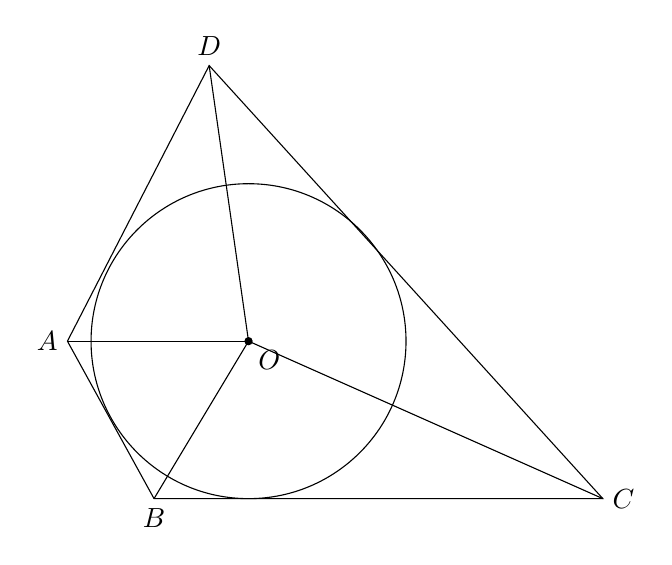
\begin{tikzpicture}
    % Define coordinates
    \coordinate (O) at (0,0);
    \coordinate (A) at (-2.3, 0);
    \coordinate (B) at (-1.2, -2);
    \coordinate (C) at (4.5, -2);
    \coordinate (D) at (-0.5, 3.5);

    % Draw the circle
    \draw (O) circle (2);

    % Draw the quadrilateral edges
    \draw (A) -- (B) -- (C) -- (D) -- (A);

    % Draw lines from center to vertices
    \draw (O) -- (A);
    \draw (O) -- (B);
    \draw (O) -- (C);
    \draw (O) -- (D);

    % Draw the center point
    \fill (O) circle (1.5pt);

    % Labels
    \node[left] at (A) {$A$};
    \node[below] at (B) {$B$};
    \node[right] at (C) {$C$};
    \node[above] at (D) {$D$};
    \node[below right] at (O) {$O$};
\end{tikzpicture}
\end{document}
